%-------------------------------------------------------------------------------
%	PACKAGES AND OTHER DOCUMENT CONFIGURATIONS
%-------------------------------------------------------------------------------

\documentclass{article}

% Packages
% Packages

% \usepackage{fancyhdr} % Required for custom headers
% \usepackage{lastpage} % Required to determine the last page for the footer
% \usepackage{extramarks} % Required for headers and footers
% \usepackage[usenames,dvipsnames]{color} % Required for custom colors
\usepackage{graphicx} % Required to insert images
% \usepackage{listings} % Required for insertion of code
% \usepackage{courier} % Required for the courier font
% \usepackage{dsfont} % For special math characters
% \usepackage{verbatim}

%\usepackage{amsmath, amssymb, bm} % For matrix notation
\usepackage[english]{babel}
\usepackage[paperwidth=8.5in,paperheight=11in,margin=1.0in]{geometry}
\usepackage{listings}
\usepackage{hyperref}
%\usepackage[cmex10]{amsmath, bm}
\usepackage{amsmath, bm}
\usepackage{blkarray}








% formatting
\pdfcompresslevel0

% ==============================================================================
% PYTHON
% ==============================================================================
\usepackage[utf8]{inputenc}

% Default fixed font does not support bold face
\DeclareFixedFont{\ttb}{T1}{txtt}{bx}{n}{12} % for bold
\DeclareFixedFont{\ttm}{T1}{txtt}{m}{n}{12}  % for normal

% Custom colors
\usepackage{color}
\definecolor{deepblue}{rgb}{0,0,0.5}
\definecolor{deepred}{rgb}{0.6,0,0}
\definecolor{deepgreen}{rgb}{0,0.5,0}

\usepackage{listings}

% Python style for highlighting
\newcommand\pythonstyle{\lstset{
language=Python,
basicstyle=\ttm,
otherkeywords={self},             % Add keywords here
keywordstyle=\ttb\color{deepblue},
emph={MyClass,__init__},          % Custom highlighting
emphstyle=\ttb\color{deepred},    % Custom highlighting style
stringstyle=\color{deepgreen},
frame=tb,                         % Any extra options here
showstringspaces=false,            % 
breaklines=true
}}


% Python environment
\lstnewenvironment{python}[1][]
{\pythonstyle\lstset{#1}
}
{}

% Python for external files
\newcommand\pythonexternal[2][]{{
\pythonstyle\lstinputlisting[#1]{#2}}}

% Python for inline
\newcommand\pythoninline[1]{{\pythonstyle\lstinline!#1!}}
% ==============================================================================
% ==============================================================================

% Margins
\topmargin=-0.45in
\evensidemargin=0in
\oddsidemargin=0in
\textwidth=6.5in
\textheight=9.0in
\headsep=0.25in

\linespread{1.1} % Line spacing

% Set up the header and footer
\pagestyle{fancy}
\lhead{\hmwkAuthorName} % Top left header
\chead{\hmwkClass\ (\hmwkClassInstructor\ \hmwkClassTime): \hmwkTitle} % Top center head
\rhead{\firstxmark} % Top right header
\lfoot{\lastxmark} % Bottom left footer
\cfoot{} % Bottom center footer
\rfoot{Page\ \thepage\ of\ \protect\pageref{LastPage}} % Bottom right footer
\renewcommand\headrulewidth{0.4pt} % Size of the header rule
\renewcommand\footrulewidth{0.4pt} % Size of the footer rule

\setlength\parindent{0pt} % Removes all indentation from paragraphs

%----------------------------------------------------------------------------------------
%	DOCUMENT STRUCTURE COMMANDS
%	Skip this unless you know what you're doing
%----------------------------------------------------------------------------------------

% Header and footer for when a page split occurs within a problem environment
\newcommand{\enterProblemHeader}[1]{\nobreak\extramarks{#1}{#1 continued on next page\ldots}\nobreak\nobreak\extramarks{#1 (continued)}{#1 continued on next page\ldots}\nobreak}

% Header and footer for when a page split occurs between problem environments
\newcommand{\exitProblemHeader}[1]{\nobreak\extramarks{#1 (continued)}{#1 continued on next page\ldots}\nobreak\nobreak\extramarks{#1}{}\nobreak}

\setcounter{secnumdepth}{0} % Removes default section numbers
\newcounter{homeworkProblemCounter} % Creates a counter to keep track of the number of problems

\newcommand{\homeworkProblemName}{}
\newenvironment{homeworkProblem}[1][Problem \arabic{homeworkProblemCounter}]{ % Makes a new environment called homeworkProblem which takes 1 argument (custom name) but the default is "Problem #"
\stepcounter{homeworkProblemCounter} % Increase counter for number of problems
\renewcommand{\homeworkProblemName}{#1} % Assign \homeworkProblemName the name of the problem
\section{\homeworkProblemName} % Make a section in the document with the custom problem count
\enterProblemHeader{\homeworkProblemName} % Header and footer within the environment
}{\exitProblemHeader{\homeworkProblemName} % Header and footer after the environment
}

% Defines the problem answer command with the content as the only argument
\newcommand{\problemAnswer}[1]{\noindent\framebox[\columnwidth, resolution=600][c]{\begin{minipage}{0.98\columnwidth, resolution=600}#1\end{minipage}}}
% Makes the box around the problem answer and puts the content inside }

\newcommand{\homeworkSectionName}{}
\newenvironment{homeworkSection}[1]{ % New environment for sections within homework problems, takes 1 argument - the name of the section
\renewcommand{\homeworkSectionName}{#1} % Assign \homeworkSectionName to the name of the section from the environment argument
\subsection{\homeworkSectionName} % Make a subsection with the custom name of the subsection
\enterProblemHeader{\homeworkProblemName\ [\homeworkSectionName]} % Header and footer within the environment
}{
\enterProblemHeader{\homeworkProblemName} % Header and footer after the environment
}



%-------------------------------------------------------------------------------
%	NAME AND CLASS SECTION
%-------------------------------------------------------------------------------

\newcommand{\hmwkTitle}{Homework 6} % Assignment title
\newcommand{\hmwkDueDate}{Saturday, Nov 1} % Due date
\newcommand{\hmwkClass}{ECE 532} % Course/class
\newcommand{\hmwkClassTime}{11:00 am} % Class/lecture time
\newcommand{\hmwkClassInstructor}{Robert Nowak} % Teacher/lecturer
\newcommand{\hmwkAuthorName}{Elijah Bernstein-Cooper} % Your name

%-------------------------------------------------------------------------------
%	TITLE PAGE
%-------------------------------------------------------------------------------

\title{\vspace{0in}
    \textmd{\textbf{\hmwkClass:\ \hmwkTitle}}\\
    \normalsize\vspace{0.1in}\small{Due\ on\ \hmwkDueDate}\\
    \vspace{0.1in}\large{\textit{\hmwkClassInstructor\ \hmwkClassTime}}
    \vspace{0.5in}}

\author{\textbf{Elijah Bernstein-Cooper}}
\date{\today} % Insert date here if you want it to appear below your name

%-------------------------------------------------------------------------------

\begin{document}

\maketitle
%\newpage

%===============================================================================
%-------------------------------------------------------------------------------
%	PROBLEM 1
%-------------------------------------------------------------------------------
\begin{homeworkProblem}

    \begin{homeworkSection}{1a}

        We partitioned the face emotion data into 8 random partitions, then for
        each permutation of using 6 partitions for training, 1 partition for
        tuning and 1 partition for testing, we computed the truncated SVD. To
        compute the truncated SVD we first took the SVD of the training data,
        then adjusted the regularization parameter, $k$, until the residual,
        $\|\bm{b} - \bm{Ax}\|^2$, was minimized. The median $k$ was 7. The
        truncated SVD was then used to compute an estimate of the error in
        prediction with the test partition. We found that for our 56
        combinations of partitions, the average predictive error in from the
        SVD was 1.9. See the code at end of homework used to complete this
        problem.

    \end{homeworkSection}

    \begin{homeworkSection}{1b}

        We partitioned the face emotion data and computed a regularized least
        squares solutions in a similar manner to \S\,1a. To compute the
        regularized least squares, we maximize $\|\bm{b} - \bm{Ax}\|^2 +
        \lambda\|x\|^2$, with the solution $\bm{\hat{x}} = (A^T A + \lambda
        I)^{-1} A^T b$. We cycle through logarithmically spaced $\lambda$ until
        our maximization is completed. The median $\lambda$ was 2. The RLS was
        then used to compute an estimate of the error in prediction with the
        test partition. We found that for our 56 combinations of partitions,
        the average predictive error in from the RLS was 1.9, similar to the
        truncated SVD predictive error.  See the code at end of homework used
        to complete this problem.

    \end{homeworkSection}

\end{homeworkProblem}
\clearpage
%===============================================================================

%===============================================================================
%-------------------------------------------------------------------------------
%	PROBLEM 2 
%-------------------------------------------------------------------------------
\begin{homeworkProblem}
    
    \begin{homeworkSection}{2a}    
    
        We attempt to derive an original signal from noisy, blurred data. We
        used the cross-validation technique to compute the regularization
        parameters of the truncated SVD, and regularized least squares (RLS)
        solutions. We also compute a simple least-squares solution of the
        signal. See Figure~\ref{fig:prob2a} for the best-estimate signals from
        each method. See the code at end of homework used to complete this
        problem.

        \begin{figure}
            
            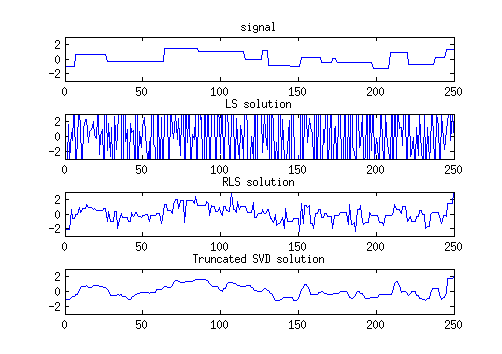
\includegraphics[width=\linewidth]{prob2a_fig.png}

            \caption{\label{fig:prob2a} The original signal plotted with the
            estimates from the least-squares, regularized least-squares, and
        truncated SVD methods of the signal.}

        \end{figure} 
    \end{homeworkSection}
    
    \begin{homeworkSection}{2b}

        We computed the 2-norms of the LS, RLS, and truncated SVD solutions for
        $\bm{\hat{x}}$ for varying values of noise strengths and averaging
        widths. See Table~\ref{table:1} for results. In general we find that
        the truncated SVD performs better than the regularized least squares
        method when comparing the estimated signal with the true signal. See
        the code at end of homework used to complete this problem.

        \begin{table}[H]

            \caption{\label{table:1} Fitting results for different averaging
            size kernels, $k$, and data noise strengths, $\sigma$. The norms of
        the LS, RLS and SVDs are all 2-norms between the blurred signal and the
    best-estimate of the blurred signal.}

            \begin{center}
                \begin{tabular}{lccc}

                    Properties & LS norm & RLS norm & SVD norm \\
                    \hline \hline
                    k = 30, $\sigma$ = 0.1 & 80 & 12.0 & 8.1 \\
                    k = 10, $\sigma$ = 0.1 & 41 & 9.5 & 7.9 \\
                    k = 50, $\sigma$ = 0.1 & 120 & 13.3 & 13.0 \\
                    k = 30, $\sigma$ = 0.01 & 9 & 6.3 & 6.7 \\
                    k = 30, $\sigma$ = 1 & 955 & 15.2 & 10.8 \\

                \end{tabular}
            \end{center}
        \end{table}

    \end{homeworkSection}
    
\end{homeworkProblem}
\clearpage
%===============================================================================

Code:

{\large \bf Problem 1a} \\
\lstinputlisting{hw6_prob1a.m} 
\hrule \hrule

{\large \bf Problem 1b} \\
\lstinputlisting{hw6_prob1b.m} 
\hrule \hrule

{\large \bf Problem 2a+b} \\
\lstinputlisting{hw6_prob2a.m}

\end{document}

